\imprimircapa
\imprimirfolhaderosto

\pagenumbering{roman}

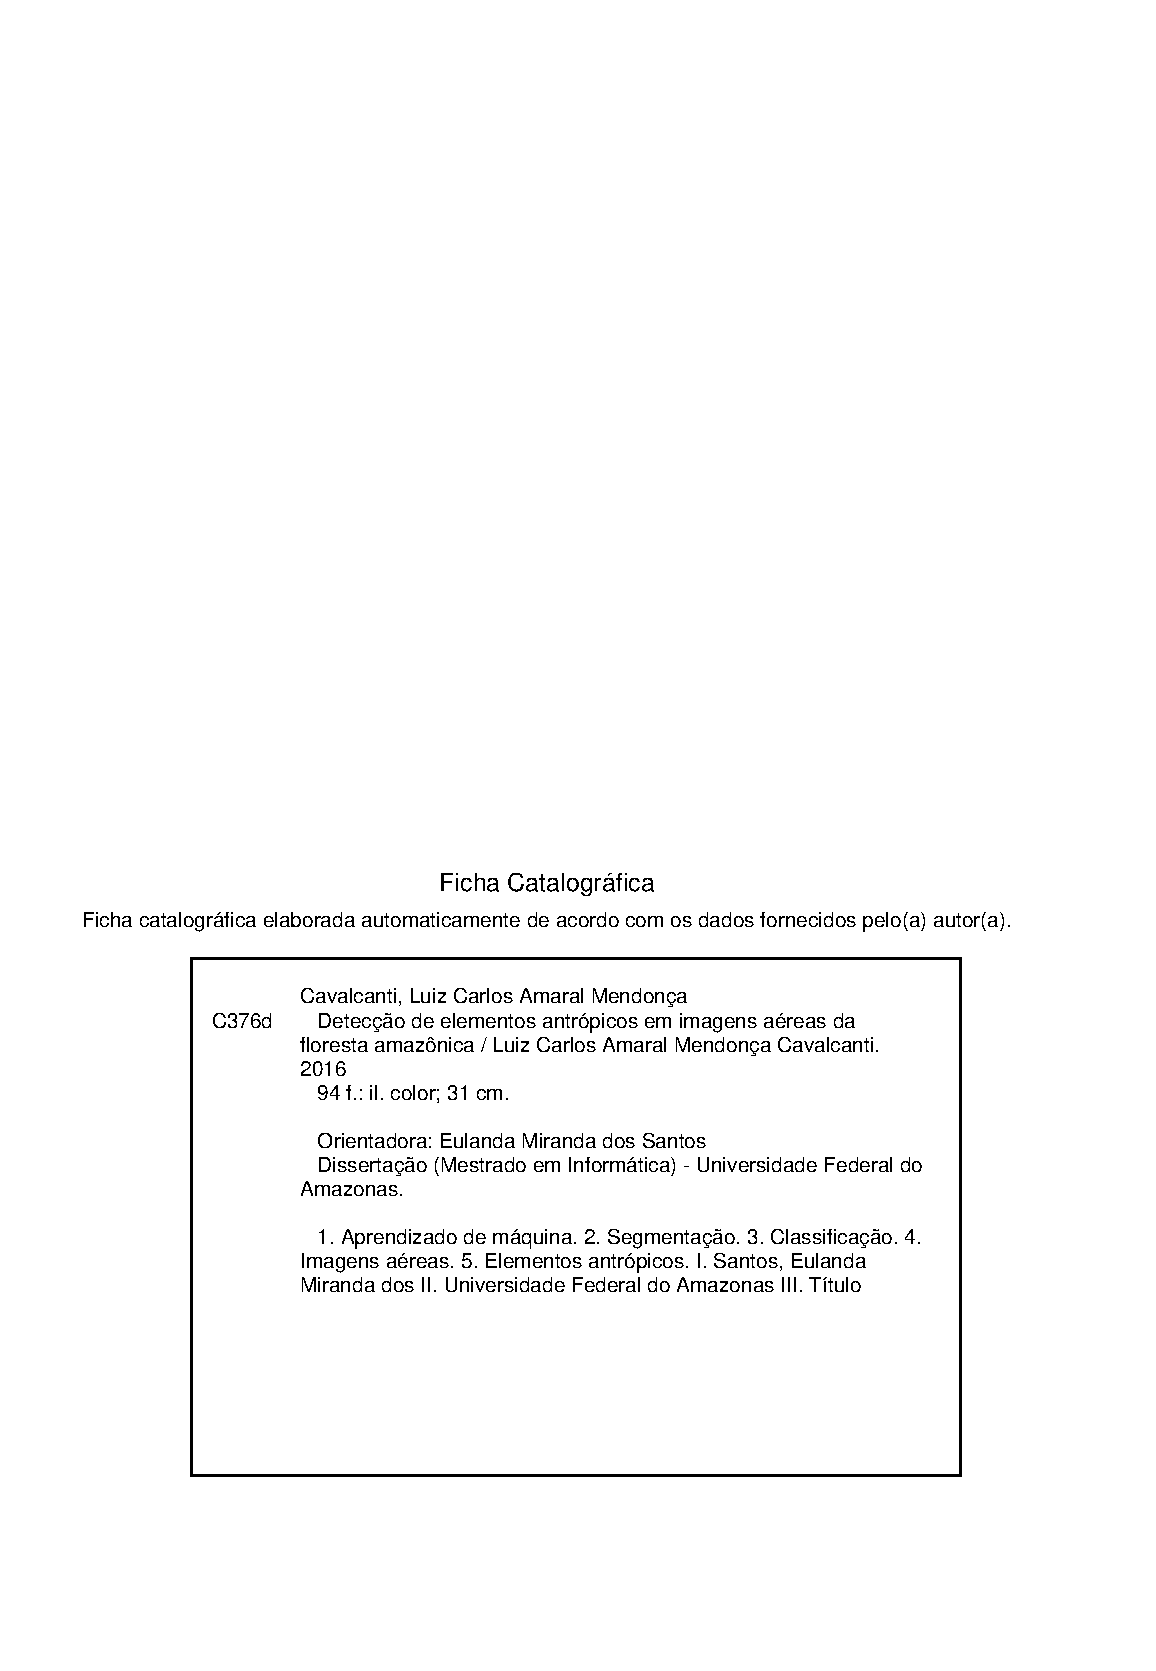
\includepdf[pages={1}]{ficha_catalografica.pdf}

\begin{folhadeaprovacao}
    \begin{center}
        {\ABNTEXchapterfont\large\imprimirautor}
        \vspace*{\fill}\vspace*{\fill}
        \begin{center}
            \ABNTEXchapterfont\bfseries\Large\imprimirtitulo
        \end{center}
        \vspace*{\fill}
    \hspace{.45\textwidth}
    \begin{minipage}{.5\textwidth}
        \imprimirpreambulo
    \end{minipage}%
    \vspace*{\fill}
    \end{center}
    Trabalho aprovado. \imprimirlocal, 1 de julho de 2016:
    \assinatura{\textbf{\imprimirorientador} \\ Presidente \\ PPGI/UFAM}
    \assinatura{\textbf{Prof. Dr. George Darmiton da Cunha Cavalcanti} \\ PGCC/UFPE}
    \assinatura{\textbf{Prof. Dr. José Reginaldo Hughes Carvalho} \\ PPGI/UFAM}
    \assinatura{\textbf{Prof. Dr. José Luiz de Souza Pio} \\ PPGEE/UFAM}

    \begin{center}
        \vspace*{0.5cm}
        {\large\imprimirlocal}
        \par
        {\large\imprimirdata}
        \vspace*{1cm}
    \end{center}
\end{folhadeaprovacao}

\begin{dedicatoria}
	\vspace*{\fill}
	À Isabel Wittmann
	\vspace*{\fill}
\end{dedicatoria}

\begin{agradecimentos}
	À professora e orientadora Dra. Eulanda Santos, pela paciência, revisões, direcionamentos e mais paciência.

	Ao Centro Gestor e Operacional do Sistema de Proteção da Amazônia (CENCIPAM), especialmente à Dra. Solange Costa pela contribuição na avaliação e validação dos resultados preliminares, sem as quais este trabalho não seria possível.

	Aos amigos do trabalho e academia, principalmente à Arthur Batista, que fora os dois durante todo o percurso.

	Aos professores Edleno Moura, Marco Cristo, Altigran Soares, José Reginaldo Hughes e José Pio pelas aulas, cobranças e acompanhamento ao longo do curso.

	À família, direta e indireta, pelo apoio vitalício.

\end{agradecimentos}

\begin{epigrafe}
	\vspace*{\fill}
	\begin{flushright}
		\textit{``As forças da natureza são máquinas infinitas, as máquinas são forças limitadas''\\Victor Hugo, Os Trabalhadores do Mar}
	\end{flushright}
\end{epigrafe}

\tableofcontents*
\clearpage

\listoffigures
\clearpage

\listoftables
\clearpage

\begin{siglas}
	\item[BSD500] Berkeley Segmentation Data Set and Benchmarks 500
	\item[CENSIPAM] Centro Gestor e Operacional do Sistema de Proteção da Amazônia
	\item[CFS] Correlation-based Feature Subset Selection
	\item[IBGE] Instituto Brasileiro de Geografia e Estatística
	\item[INPE] Instituto Nacional de Pesquisas Espaciais
	\item[FSEG] Factorisation-Based Segmentation
	\item[GCE] Global Consistency Error
	\item[HSV] Hue-Saturation-Value
	\item[JPEG] Joint Photographic Experts Group
	\item[JSEG] J Segmentation
	\item[KNN] K-Nearest Neighbours
	\item[LBP] Local Binary Pattern
	\item[LBP-HF] Local Binary Pattern Histogram Fourier
	\item[LCE] Local Consistency Error
	\item[LIDAR] Light Detection and Ranging
	\item[MoG] Mixture of Gaussians
	\item[MSEG] Multi-resolution Region Merging Segmentation
	\item[OCNN] One-Class Nearest Neighbours
	\item[OC-SVM] One-Class Support Vector Machines
	\item[PDI] Processamento Digital de Imagens
	\item[RADAR] Radio Detection and Ranging
	\item[ROC] Receiver Operating Characteristic
	\item[SCSVDD] Spatial-Contextual Support Vector Domain Description
	\item[SRM] Statistical Region Merging
	\item[SVDD] Support Vector Domain Description
	\item[SVM] Support Vector Machines
	\item[UAV] Unmanned Aerial Vehicle
	\item[VANT] Veículo Aéreo Não-Tripulado
\end{siglas}


\pagenumbering{arabic}